%
% Complete documentation on the extended LaTeX markup used for Insight
% documentation is available in ``Documenting Insight'', which is part
% of the standard documentation for Insight.  It may be found online
% at:
%
%     http://www.itk.org/

\documentclass{InsightArticle}

\usepackage[dvips]{graphicx}
\usepackage{tabularx}
%%%%%%%%%%%%%%%%%%%%%%%%%%%%%%%%%%%%%%%%%%%%%%%%%%%%%%%%%%%%%%%%%%
%
%  hyperref should be the last package to be loaded.
%
%%%%%%%%%%%%%%%%%%%%%%%%%%%%%%%%%%%%%%%%%%%%%%%%%%%%%%%%%%%%%%%%%%
\usepackage[dvips,
bookmarks,
bookmarksopen,
backref,
colorlinks,linkcolor={blue},citecolor={blue},urlcolor={blue},
]{hyperref}


%  This is a template for Papers to the Insight Journal. 
%  It is comparable to a technical report format.

% The title should be descriptive enough for people to be able to find
% the relevant document. 
\title{An ITK Implementation of a Diffusion Tensor Images Resampling Filter}

% 
% NOTE: This is the last number of the "handle" URL that 
% The Insight Journal assigns to your paper as part of the
% submission process. Please replace the number "1338" with
% the actual handle number that you get assigned.
%
\newcommand{\IJhandlerIDnumber}{3189}

% Increment the release number whenever significant changes are made.
% The author and/or editor can define 'significant' however they like.
\release{1.00}

% At minimum, give your name and an email address.  You can include a
% snail-mail address if you like.
\author{Francois Budin$^{1}$, Sylvain Bouix$^{2}$, Martha Shenton$^{2}$, Martin Styner$^{1}$, Ipek Oguz$^{1}$}
\authoraddress{$^{1}$Department of Psychiatry, University of North Carolina, Chapel Hill, NC\\
               $^{2}$Psychiatry Neuroimaging Laboratory, Department of Psychiatry, Brigham and Women's Hospital, Harvard Medical School, Boston MA}

\begin{document}

%
% Add hyperlink to the web location and license of the paper.
% The argument of this command is the handler identifier given
% by the Insight Journal to this paper.
% 
\IJhandlefooter{\IJhandlerIDnumber}


\ifpdf
\else
   %
   % Commands for including Graphics when using latex
   % 
   \DeclareGraphicsExtensions{.eps,.jpg,.gif,.tiff,.bmp,.png}
   \DeclareGraphicsRule{.jpg}{eps}{.jpg.bb}{`convert #1 eps:-}
   \DeclareGraphicsRule{.gif}{eps}{.gif.bb}{`convert #1 eps:-}
   \DeclareGraphicsRule{.tiff}{eps}{.tiff.bb}{`convert #1 eps:-}
   \DeclareGraphicsRule{.bmp}{eps}{.bmp.bb}{`convert #1 eps:-}
   \DeclareGraphicsRule{.png}{eps}{.png.bb}{`convert #1 eps:-}
\fi


\maketitle


\ifhtml
\chapter*{An ITK Implementation of a Diffusion Tensor Images resampling filter\label{front}}
\fi


% The abstract should be a paragraph or two long, and describe the
% scope of the document.
\begin{abstract}
\noindent
This paper describes the implementation of a resampling filter for Diffusion Tensor Images (DTI) in the Insight ToolKit (ITK). ITK already contains a filter for resampling scalar and vector images as well as several transformation and interpolation classes. However, due to the directional nature of DT images, using the existing classes would result in losing the structural information of the image.

We developed a new resampling filter, specific to DTI, that preserves the structure by applying a rotation directly on the tensors while performing the transformation of the image. New transformation and interpolator classes have also been implemented to handle tensors correctly. The new transformation classes are based on algorithms described by D.C. Alexander et al. \cite{Alexander2001}. Finally, three filters have been written to correct symmetric semi-definite matrices that would no longer be positive after the resampling process and project them into the tensors' space. In addition, a software based on the new classes has been developed and is provided with this article.
\end{abstract}

\IJhandlenote{\IJhandlerIDnumber}

\tableofcontents

\section{Introduction}

Diffusion Tensor Imaging (DTI) \cite{Basser1994} is an image modality that measures the motion of water molecules in tissue and models this motion with a diffusion tensor (a symmetric positive semi-definite matrix, which can be visualized as an oriented ellipsoid). The size, orientation and anisotropy of the diffusion tensor at each voxel in the image, as well as the analysis of its eigen system have been extremely useful in the study of several diseases including chronic and acute cerebral ischemia, multiple sclerosis, metabolic disorders, epilepsy, and brain tumors \cite{Dong2004}.

Before analyzing images, one often needs to realign them to bring them into a common coordinate frame: a resampling filter is used to obtain the transformed image. For scalar images, the filter computes the position of a voxel after transformation and interpolates the value at that position. No additional step is performed to modify the value of the voxel. If a resampling filter for scalar images is applied to a DT image, tensors will conserve their original orientation in the output image. Therefore, if a rotation is applied to the image, the structure in the output image will be lost. One needs to transform the tensors themselves along with the image to preserve its coherence.

The Insight ToolKit (ITK) library \cite{ITKSoftwareGuideSecondEdition} contains filters to resample scalar and vector images but none for DT images. In this paper we present the implementation of a filter in the ITK framework to resample DT images as well as transformation and interpolation classes that can be used with it. The transformations are based on algorithms described by D.C. Alexander et al. \cite{Alexander2001}. Additionally, classes have been created to correct transformed tensors that are no longer positive semi-definite. Software based on these classes has been developed and is provided with this paper to allow the reader comparisons between the different transformation and interpolation algorithms.

\section{Theory}
\subsection{Transformation}

Transforming scalar images consists of computing the new position of a voxel after applying a given transformation to it. Using a backward transformation, one computes for each voxel of the output image its corresponding position in the input image and assigns its intensity by interpolating values in the source image. However, for DT images a second step is necessary to preserve the relative orientation of the tensor with respect to the image coordinate system. If a rotation is applied to the image, the tensors have to be rotated as well so that the diffusion orientation information in the image is still valid. Since backward transformations are used, the inverse rotation (transpose matrix) has to be used for the tensors.

In the general case, applying the transformation $M$ to a matrix $D$ is given by equation (\ref{eq:MatrixRotation}). In the case of a rotation $R$, the general formula becomes equation (\ref{eq:TensorRotation}).
\begin{align}
\label{eq:MatrixRotation}
D &= M \cdot D \cdot M^{-1}\\
\label{eq:TensorRotation}
D &= R \cdot D \cdot R^{T}
\end{align} 

If the transformation is not a rotation, one cannot apply it directly as this would modify the size and the shape of the tensors and misrepresent the diffusion properties of the underlying tissue. Only the tensor orientation should be modified. In the case of affine transformations, Alexander et al. \cite{Alexander2001} suggested two different strategies to find the tensors' rotation matrix: the Finite Strain (FS) and the Preservation of Principal Direction (PPD).

\subsubsection{Finite Strain Method}
Any non-singular matrix $F$ can be decomposed into a rigid rotation component $R$ and a deformation component $U$ where
\begin{gather}
F = U \cdot R\\
R = (F \cdot F^{T} )^{-{1/2}} \cdot F
\end{gather}

$R$ is used to transform the tensors. The rotation matrix needs to be extracted from the transformation matrix only once for the whole image.

However some problems might arise from the use of this method. To illustrate this, a shearing deformation has been applied on a synthetic image. The results are visible in  Figure \ref{fig:FSTransformation}. These images show that this method is not optimal because the image structure is not always well preserved. When applying a horizontal shearing (Fig. \ref{fig:FSTransformation}b) to the phantom image (Fig. \ref{fig:FSTransformation}a), the tensors should not be transformed. On the other hand, when applying a vertical shearing on the image(Fig. \ref{fig:FSTransformation}c), the tensors should be rotated with a larger angle.

%\begin{figure}
%\center
%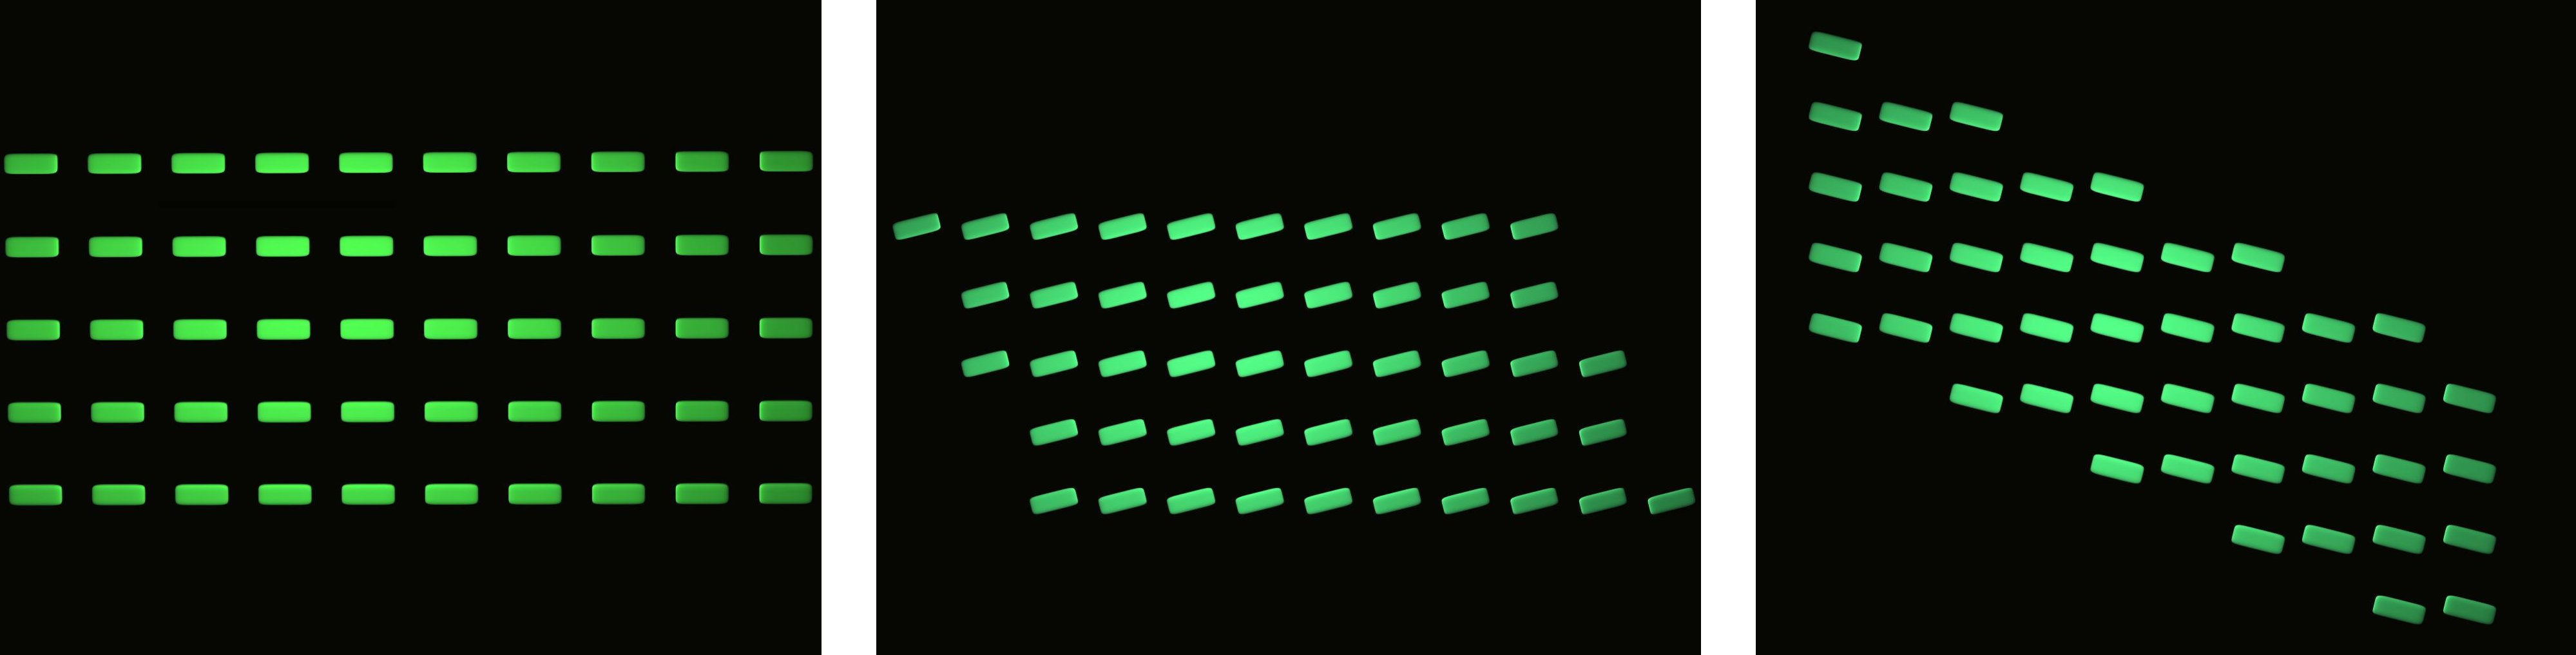
\includegraphics[width=0.95\textwidth]{plan2dyz-skew-noppd-attached.jpg}
%\itkcaption[Tensor Transformation]{Finite Strain Method. From left to right: a) Diffusion Tensor Image %phantom. b) Horizontal shearing applied to DTI phantom. c) Vertical shearing applied to DTI phantom}
%\label{fig:FSTransformation}
%\end{figure}

\begin{figure}
\newcolumntype{C}{>{\centering\arraybackslash}X }
\begin{tabularx}{\textwidth}{CCC}
(a) & (b) & (c) \\
\multicolumn{3}{c}{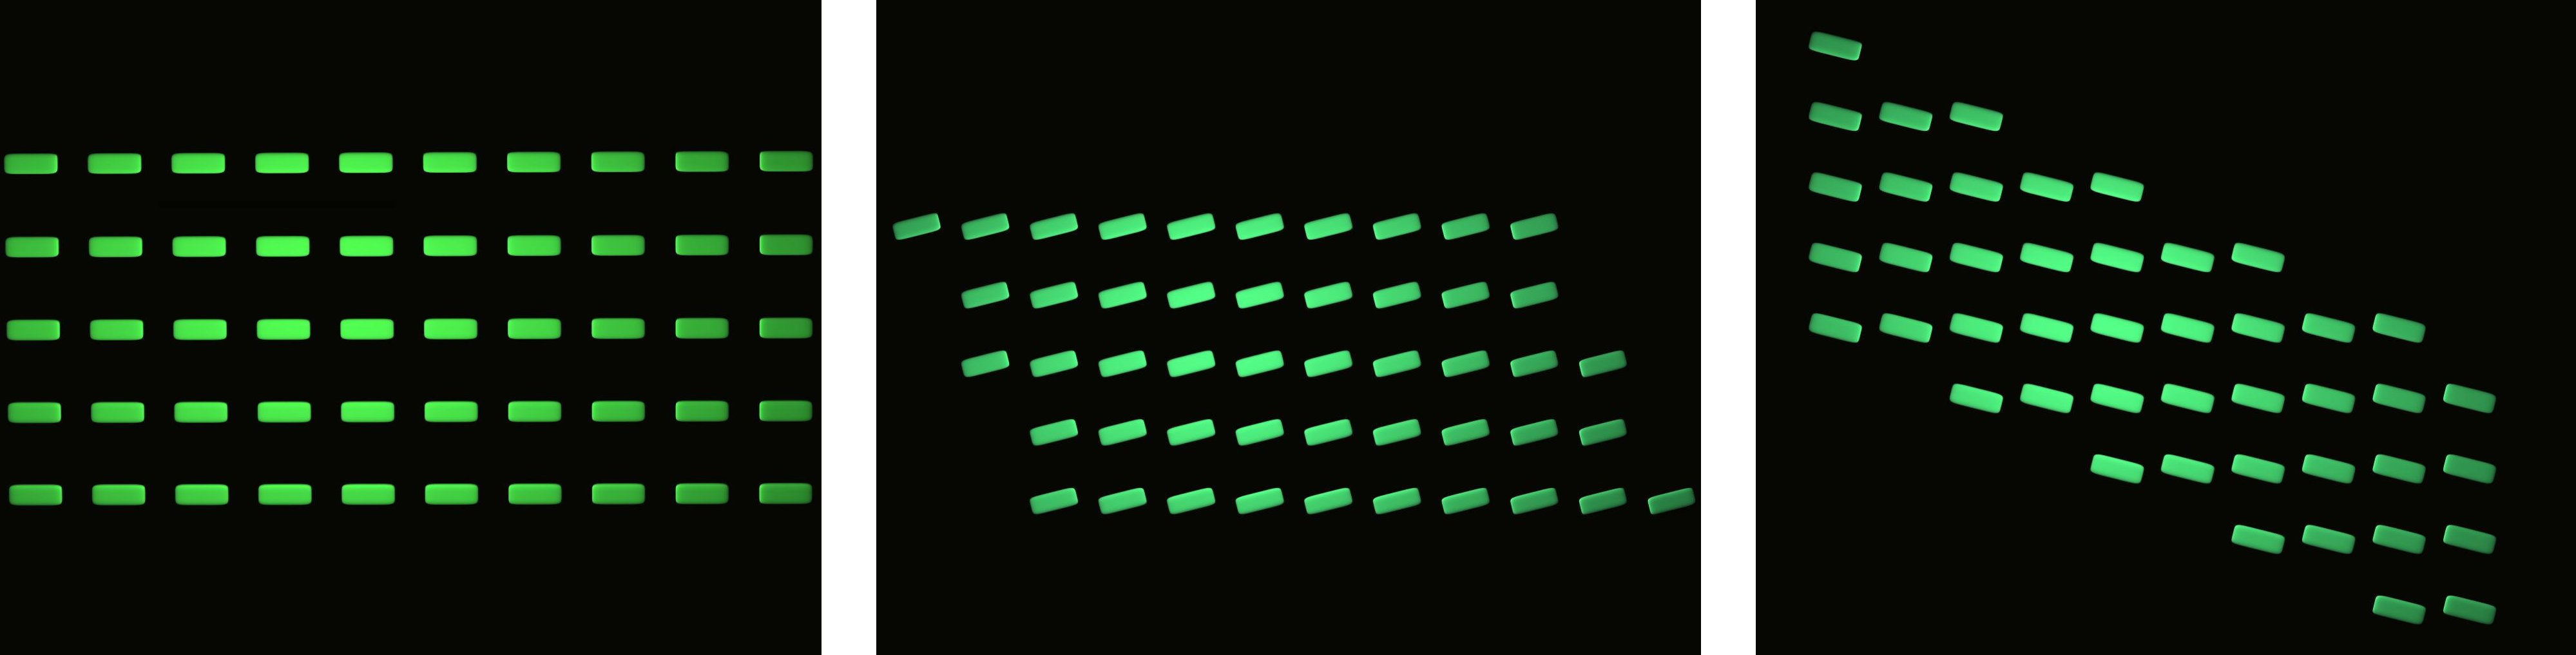
\includegraphics[width=0.95\textwidth]{plan2dyz-skew-noppd-attached.jpg} }\\
\end{tabularx}
\itkcaption[Tensor Transformation]{Finite Strain Method. From left to right: a) Diffusion Tensor Image phantom. b) Horizontal shearing applied to DTI phantom. c) Vertical shearing applied to DTI phantom}
\label{fig:FSTransformation}
\end{figure}


\subsubsection{Preservation of Principal Direction Method}
To overcome the problems that appear using FS, one can use the Preservation of Principal Direction (PPD) method. In this method, the transformation applied to the tensors has to be recomputed for each tensor of the image as the amount of rotation is dependent on the orientation of the tensor (see Fig. \ref{fig:FSTransformation}b,c).

In our experiments on a phantom image (Fig. \ref{fig:PPDTransformation}b, \ref{fig:PPDTransformation}c), the structure of the image is well preserved with this method.  However, Alexander et al. \cite{Alexander2001} also noted that the FS method gives very similar results to PPD when applied to real biological tissue images and thus might be more advantageous for computational efficiency.

\begin{figure}
\newcolumntype{C}{>{\centering\arraybackslash}X }
\begin{tabularx}{\textwidth}{CCC}
(a) & (b) & (c) \\
\multicolumn{3}{c}{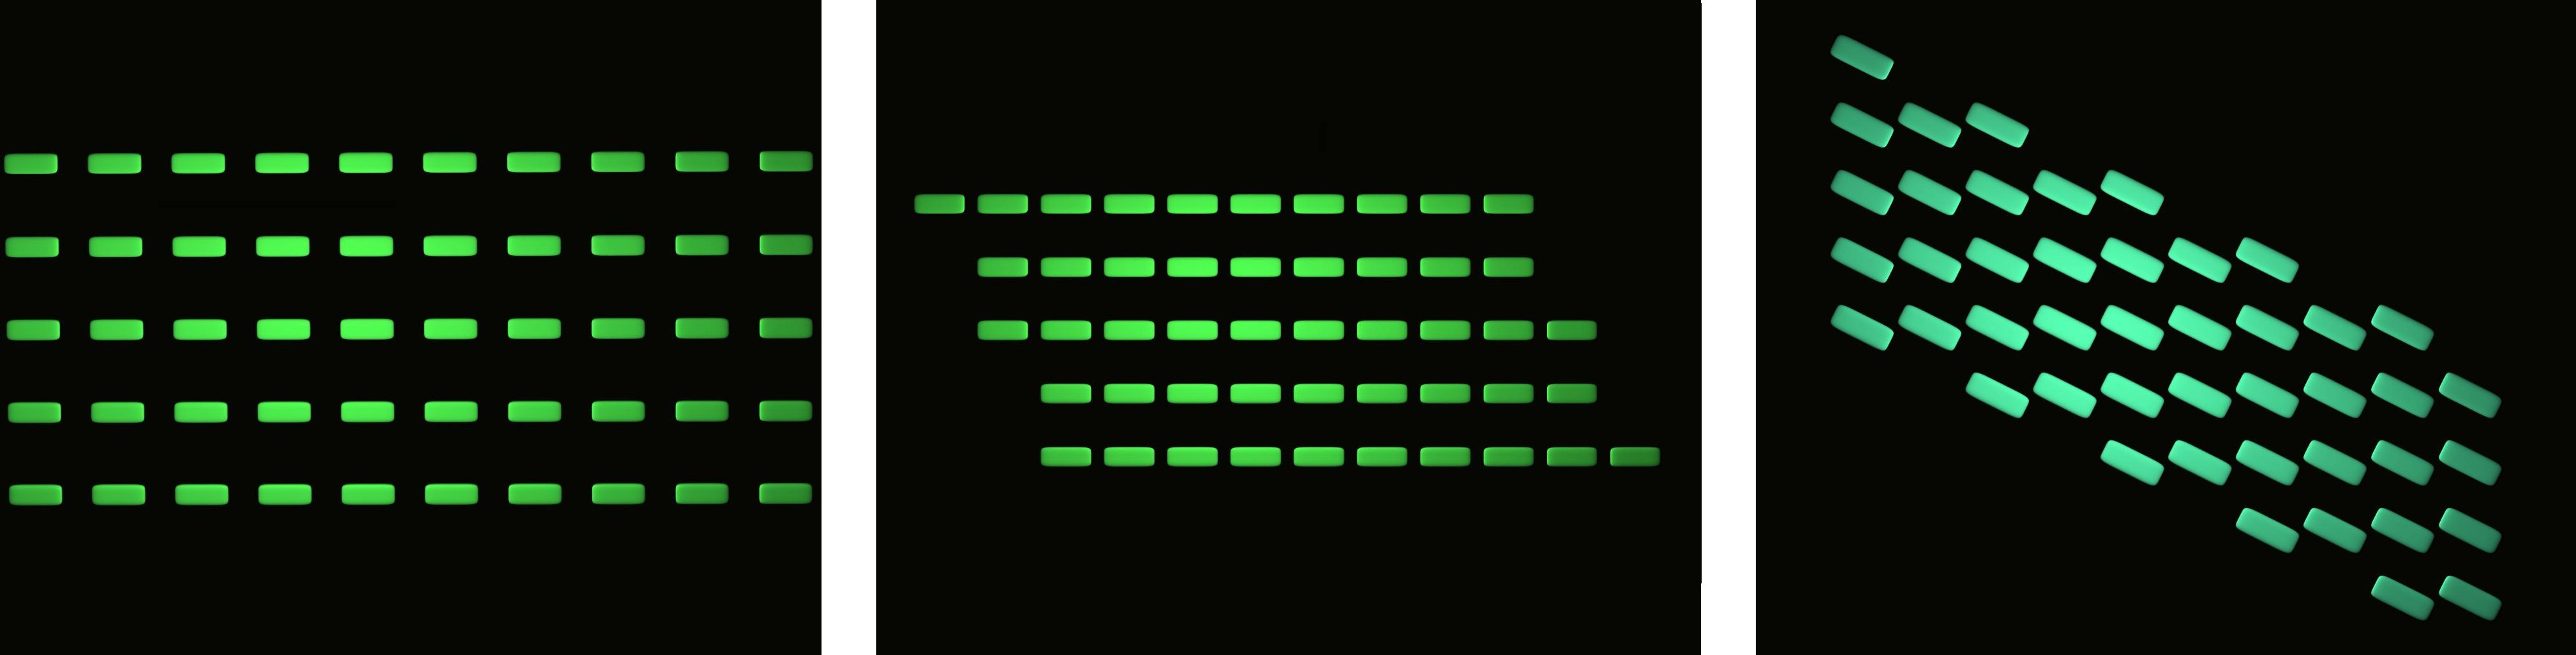
\includegraphics[width=0.95\textwidth]{plan2dyz-skew-ppd-attached.jpg} }\\
\end{tabularx}
\itkcaption[Tensor Transformation]{Preservation of Principal Direction Method. From left to right: a) Diffusion Tensor Image phantom. b) Horizontal shearing applied to DTI phantom. c) Vertical shearing applied to DTI phantom}
\label{fig:PPDTransformation}
\end{figure}


\subsubsection{Non-Rigid Transformations}
Alexander et al. have also shown how to transform DT images with higher order transformations. The extension of the method is straightforward. An image transformation can be expressed as a displacement field u(x) so that at each position x of the image, $T(x) = x + u(x)$. An affine transformation $T$ can be described by $T(x) = F x + t$. Differentiating these two expressions with respect to $x$ gives $T'(x) = I + J_{u}$ and $T'(x) = F$ where $I$ is the identity matrix and $J_{u}$ is the Jacobian of the displacement field $u$. A local affine model of a more complex transformation can be created by taking $F = I + J_{u}$ at every point. One can then use one of the two methods described previously (FS or PPD) to compute the transformed tensors.

\subsection{Interpolation}
The transformation results in the need to evaluate the image at non-grid locations. An interpolator is used to compute the values at these non-discrete positions. Several interpolation methods have been developed for scalar images (e.g. nearest neighbor, linear, cubic, BSpline) \cite{Meijering2002,Meijering2000,Meijering2003}. As DTI is a multicomponent image, we implemented two basic techniques, 1) Nearest neighbor interpolation and 2) Component-wise scalar interpolation (i.e. each component of the tensor gets interpolated independently using a standard scalar interpolation technique).

The nearest neighbor interpolation for tensor images is equivalent to the one for scalar images. The tensor of the closest voxel from the transformed point is copied into the new location. Using this method, there is no risk to obtain a matrix that does not belong to the tensor space, but images can appear "blocky".

Component-wise interpolation consists of interpolating each component of the tensor individually. In this case, the tensor image is separated into six different images composed, at each voxel, of one tensor component. Standard scalar interpolation techniques can then be applied (Fig. \ref{fig:InterpolationIso},\ref{fig:InterpolationProlate}). We have implemented three types of interpolator: linear, BSpline and windowed sinc.

\begin{figure}
\center
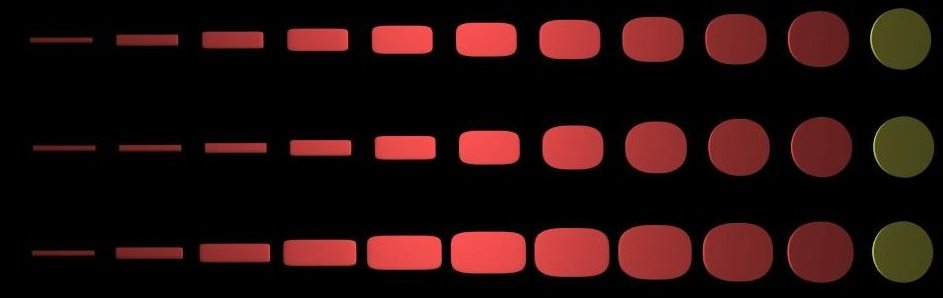
\includegraphics[width=0.8\textwidth]{2tensorsPhantom2-iso(linear-bs-ws).jpg}
\itkcaption[Tensor Interpolation]{Interpolation between one prolate and one oblate tensors. From
top to bottom: linear, BSpline order 2, windowed sinc with Welch kernel interpolator.\\}
\label{fig:InterpolationIso}
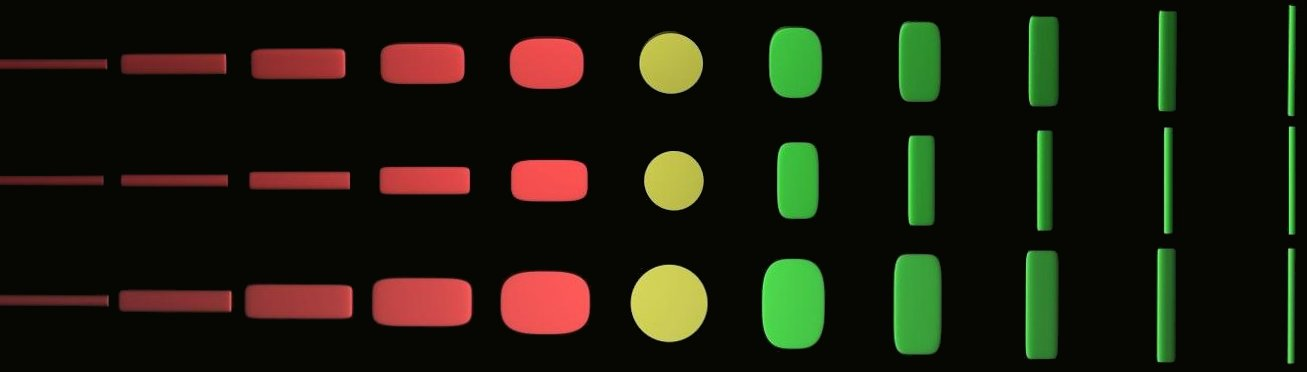
\includegraphics[width=0.8\textwidth]{2tensorsPhantom2(linear-bs-ws).jpg}
\itkcaption[Tensor Interpolation]{Interpolation between two prolate tensors. From top to bottom:
linear, BSpline order 2, windowed sinc with Welch kernel interpolator.}
\label{fig:InterpolationProlate}
\end{figure}

\subsection{Tensor Correction}
Diffusion tensors (positive semi-definite matrices) form a convex half-cone in the vector space of matrices and simple arithmetic operations with tensor components can lead to non-positive semi-definite matrices, thus illegal diffusion tensors.
Some of the previously presented interpolators may generate such invalid tensors, in particular the positivity of the matrix may not be preserved.

To move the interpolated matrix back into the space of diffusion tensors, three correction methods have been implemented:
\begin{itemize}
\item Set negative eigenvalues to zero 
\item Set negative eigenvalues to their absolute value 
\item Set the matrix representing the tensor to the nearest symmetric positive semi-definite matrix (eq. \ref{eq:ClosestMatrix}) as defined by Higham \cite{Higham1988}. $X$ is the nearest symmetric positive semi-definite matrix to $A$ in the Frobenius norm, $B$ is the symmetric part of $A$ (eq. \ref{eq:sym}) and $H$ is the symmetric polar factor of $B$ (eq. \ref{eq:polar}).
\begin{align}
\label{eq:ClosestMatrix}
X &= (B + H )/2\\
\label{eq:sym}
B &= (A + A^{T} )/2\\
\label{eq:polar}
H &= \sqrt{ B^{T} \cdot B }
\end{align}

\end{itemize}

\section{Implementation}


\subsection{Organization of the Software}
A global execution diagram of the software is shown in Figure \ref{fig:SoftwareExecutionDiagram}. It shows the organization of the different components of the resampling program. The transforms both evaluate the new tensor position and transform the tensor after the interpolation. The resampling filter executes this process for every voxel of the output image.

\begin{figure}
\center
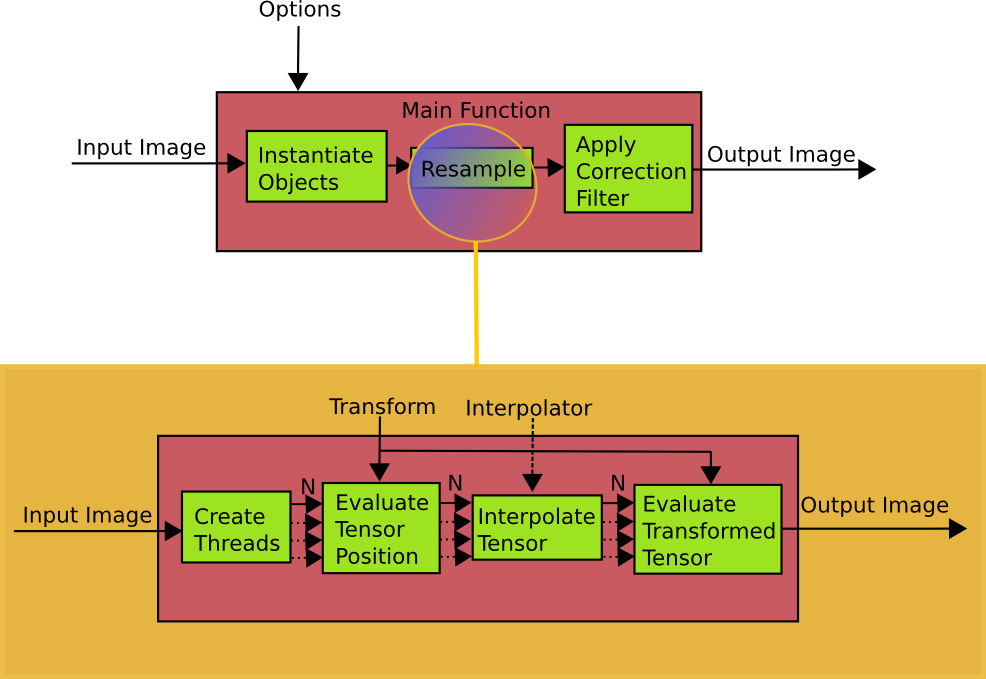
\includegraphics[width=0.75\textwidth]{Program.png}
\itkcaption[Tensor Transformation]{Software execution diagram}
\label{fig:SoftwareExecutionDiagram}
\end{figure}


\subsection{Diffusion Tensor Resampling Filter}
\code{itk::DiffusionTensor3DResample} has been implemented as a subclass of \code{itk::ImageToImageFilter}. It has a similar structure to \code{itk::ResampleImageFilter}. Hence it should be trivial to modify a software using the latter class and replace it with the Diffusion Tensor resampling filter one.

The main methods of this class are \code{SetInput()}, \code{SetInterpolator()} and \code{SetTransform()}.

\subsection{Transforms}
Three main types of transforms have been implemented: \code{itk::DiffusionTensor3DRigidTransform}, \code{itk::DiffusionTensor3DAffineTransform} and \code{itk::DiffusionTensor3DNonRigidTransform}.

Two subclasses of \code{itk::DiffusionTensor3DAffineTransform} have been implemented: one for the Finite Strain (FS) strategy and one for the Preservation of the Principal Direction (PPD) strategy. Any kind of transformation supported in ITK (for which the computation of the Jacobian is properly implemented) can be loaded in \code{itk::DiffusionTensor3DNonRigidTransform} and used to transform a DTI.

\subsection{Interpolators}

Interpolators available in ITK for scalar images cannot be used with tensor images. These interpolators are subclasses of \code{itk::InterpolateImageFunction}, itself a subclass of \code{itk::ImageFunction}. It is not possible to create a class derived from \code{itk::InterpolateImageFunction} for tensor images due to an implementation incompatibility. To keep the structure of the new interpolators as close as possible to the structure of the existing ones, the tensor interpolator base class has been implemented as a derived class of \code{itk::ImageFunction}. This allows the access to the method \code{IsInsideBuffer()} necessary for the resampler to know whether it should  interpolate a tensor at that position or whether the current point is outside the image.

\code{itk::DiffusionTensor3DNearestNeighborInterpolateFunction} is simply a re-implementation for tensors of \code{itk::NearestNeighborInterpolateImageFunction} available in ITK.
The other tensor interpolation classes that have been developed are wrappers for the original interpolation classes in ITK. The 6 components of the tensors need to be separated into 6 images. For this purpose, \code{itkSeparateComponentsOfADiffusionTensorImage}, a multithreaded filter, was created. Once the component separation done, the ITK scalar interpolators can be used for each component of the tensors through our new classes.

\subsection{Extending Existing ITK Classes}
	
To resample DT Images, it is necessary to multiply the tensors by a rotation matrix. This operation is not currently available in \code{itk::DiffusionTensor}. A subclass of \code{itk::DiffusionTensor} called \code{itk::DiffusionTensor3DExtended} was created to be able to get a matrix from a tensor. One can then multiply this matrix and convert it back to a tensor.

It is also not possible to directly cast matrices with scalar values of one type into matrices with another scalar type using \code{itk::Matrix}. All the transformation operations are performed with doubles. Hence it is necessary to convert the components of the matrices obtained from the tensors to doubles; \code{itk::MatrixExtended} has been implemented to allow that operation.

\subsection{Warp Transformations}

ITK contains a warping filter (\code{itk::WarpImageFilter}) which allows to apply a deformation field to an image. However, there is currently no warp transformation available which could be set as a transformation in a resampling filter. A new class (\code{itk::WarpTransform3D}) was implemented to transform a point using a deformation field and compute the Jacobian of the field at a given position.

In the case of multiple transformations in a row, if these are applied sequentially, there will be as many interpolations as there are transformations. Each time this is done, some error will be introduced in the image. To avoid this, one can concatenate all the transformations into one deformation field and reduce the number of interpolations to one.

\code{itk::TransformDeformationFieldFilter} was implemented to combine all the transformations into a single deformation field. This filter takes an input field and compute the new field after a second transformation is added. The initial deformation field can be set to the identity transformation, which corresponds to setting the whole deformation field to vectors filled with 0, if there is no initial deformation field.


\section{Performance}
\subsection{Computational Time}

One important question when processing images is the computational time. The perfomance of the provided software was tested on a DT image of 512x256x256 voxels. The computer used has an Intel Xeon X5570 (2.93GHz, 4 cores) processor and 6GB (DDR3 at 1333MHz) of memory. Since the resampling filter is multithreaded, the more processors/cores the computer has, the faster the program will be.

Loading and saving the image takes about 30 seconds. A correction filter is applied after the resampling process and takes approximately 28 seconds. Applying a rigid transformation takes approximately the same amount of time as applying an FS affine transformation (Fig. \ref{fig:ResamplingTime}). The only difference is that the tensors' rotation matrix has to be extracted once at the beginning of the process for the FS affine transformation. The computational time difference between an affine transformation using the FS method and one using the PPD method is small. The time difference between each try is induced mostly by the kind of interpolation used. Applying a BSpline transformation, however, also makes the resampling process much slower, whether it is with a bulk\footnote{A bulk transform is a second transform associated to the BSpline one. Both deformations are computed from the original point position. Both displacement vectors are added to compute the transformed point position.} affine transformation or merged in a deformation field with a separate affine transformation. The choice of the interpolator significantly affects the computational time for rigid and affine transforms. For more complex transforms, the computational time due to the interpolator is proportionally less important.

\begin{figure}
\center
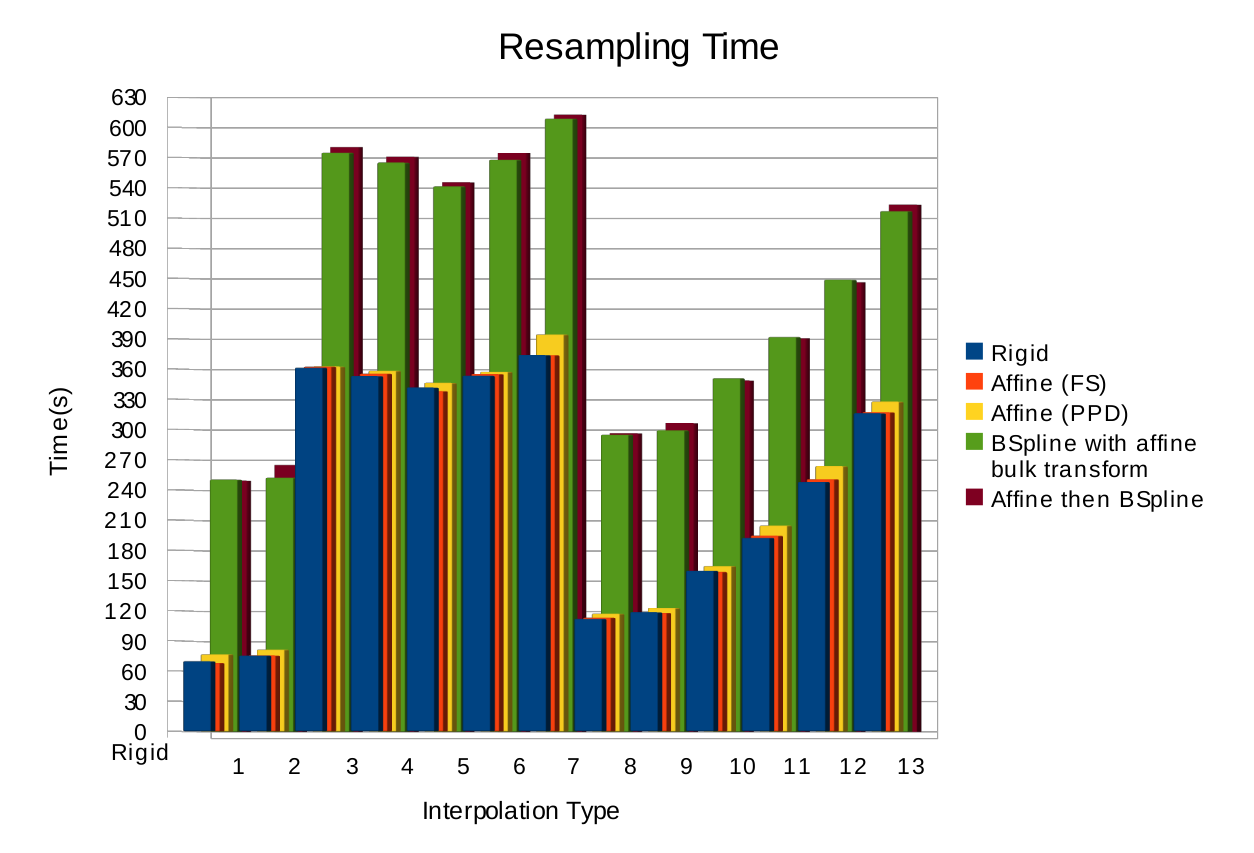
\includegraphics[width=0.95\textwidth]{Screenshot-results-graph3.png}
\itkcaption[Resampling Time]{Computational Time; 1: Nearest neighbor; 2: Linear; 3 to 7: windowed sinc using various kernels (Hamming, Cosine, Welch, Lanczos, Blackman); 8 to 13: BSpline with various orders (0 to 5)}
\label{fig:ResamplingTime}
\end{figure}

\subsection{Memory Usage}
The amount of memory used to resample a DTI image can be important. A coarse summary of the memory usage for a 512x256x256 float input and output DTI is presented in Table \ref{table:mem}. In the case of a deformation field transformation using a BSpline interpolation, the memory usage is around 3.8GB. One should be careful that enough memory is available on the computer before starting the resampling process.

\begin{table}
\begin{tabular}{|r|l|}
  \hline
  \multicolumn{2}{|c|}{Images}\\
  \hline
  Input image & 768MB \\
  Output image & 768MB \\
  \hline
  \multicolumn{2}{|c|}{Interpolators}  \\
  \hline
  Nearest Neighborhood & No additional memory used \\
  Linear, BSpline and Windowed Sinc & 768MB (input image size) to separate\\
   & the components of the tensors into different images\\
  BSpline & Additional 768MB (input image size) for the\\
  & \code{itk::BSplineDecompositionImageFilter} \\
  & used in the BSpline interpolator.\\
 \hline
 \multicolumn{2}{|c|}{Deformations}\\
 \hline
 Deformation field & 768MB\\
 Other transformations& Small amount of memory used\\
 \hline
\end{tabular}
\caption{Coarse summary of the memory usage for a 512x256x256 float input DTI}
\label{table:mem}
\end{table}



\section{Testing}
ITK provides a class to compare images which allows to verify that the result obtained corresponds to what was expected. However, this class does not allow the comparison between two DT images. A new filter called \code{itk::DifferenceDiffusionTensor3DImageFilter} was developed to compare DT images based on \code{itk::DifferenceImageFilter}. It computes the difference between two images: at each voxel, it adds the absolute value of the difference of each component of the tensors in both images and compares this sum with a given threshold.

\code{itkTestMainExtended.h} was created, based on \code{itkTestMain.h}. It handles both scalar images and DTI. Finally, several tests were written to compare the output of our software after applying different transformations and interpolations, with reference images.



\section{Conclusion}
This paper presented newly implemented classes to resample DT images based on the ITK framework.
The resampling operation can also be done in the Log-Euclidean domain \cite{Arsigny2006}. In this case, the logarithm of the input image is computed beforehand and set as the input of the resampling filter. The exponential of the filter output is then computed. With this method, the resampled image contains only positive symmetric semi-definite matrices, and therefore there is no need to apply any correction filter to it.

The DTI resampling software provided with this paper is a module available in 3D Slicer \cite{Pieper2004}, a free open source visualization and image computing software. It integrates all the transformation classes and all the interpolation classes described in this document. The previously described software has been used to resample real images and some results are shown in appendix \ref{sec:resultsOnRealImages}.

\section{Acknowledgments}
This work was funded by the National Institutes of Health through the NIH Roadmap for Medical Research grant U54 EB005149, the NIH Program Project IP01DA022446-02, the UNC Neurodevelopmental Disorders Research Center HD 03110, the NIH STTR grant R41 NS059095 and the NIH grant RC1AA019211. I am thankful to Clement Vachet for his technical support. I am also grateful to Steve Pieper, Jim Miller and Dominik Meier for their insighful discussions and Ashley Rumple for her helpful suggestions.

The Log-Euclidean framework is protected by a patent: for any commercial use, please contact \verb\{Vincent.Arsigny, Xavier.Pennec, Nicholas.Ayache}@Sophia.Inria.fr. 
For non-commercial use, this software is free and open-source.
%The Log-Euclidean framework is protected by a patent: for any commercial use, please contact \verb\{Vincent.Arsigny,Xavier.Pennec,Nicholas.Ayache}@Sophia.Inria.fr

\section{Software Requirements}

You need to have the following software installed:

% The {itemize} environment uses a bullet for each \item.  If you want the 
% \item's numbered, use the {enumerate} environment instead.
\begin{itemize}
  \item  Insight Toolkit 3.X
  \item  CMake 2.6
\end{itemize}
For the provided DTI resampling software to pass all the verification tests successfully, the Insight Toolkit needs to be compiled with the option \code{ITK\_USE\_OPTIMIZED\_REGISTRATION} turned \code{ON}. When compiling in Release mode under Microsoft Windows, don't forget to compile ModuleDescriptionParser in Release mode before (in \$\{BINARY\_DIR\}\textbackslash GenerateCLPDirectory\textbackslash ModuleDescriptionParser).

To recompile this LaTeX file, type: \code{make -i}
%
% The preceding sections will have been written in a gentler,
% introductory style.  You may also wish to include a reference
% section, documenting all the functions/exceptions/constants.
% Often, these will be placed in separate files and input like this:

\clearpage

\appendix

\section{Appendix - Results on Real Images}

\label{sec:resultsOnRealImages}
\begin{figure}[ht]
\begin{minipage}[b]{0.5\linewidth}
\centering
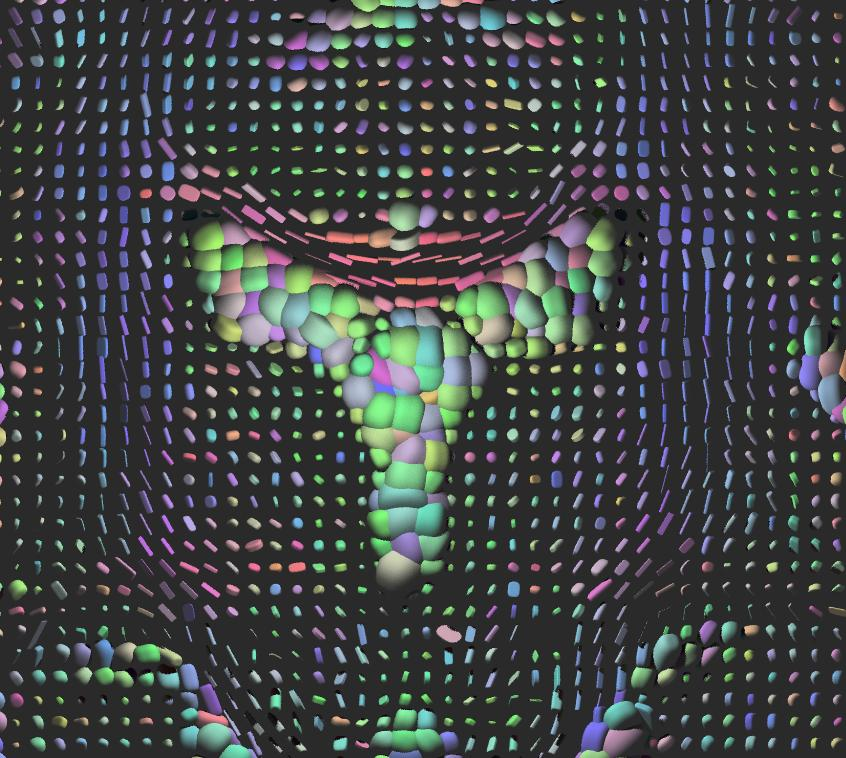
\includegraphics[width=.95\textwidth]{OriginalSlice.jpg}
\caption[Tensor Transformation]{Slice extracted from a real DT image - No transformation.\\}
\label{fig:figure1}
\end{minipage}
\hspace{0.5cm}
\begin{minipage}[b]{0.5\linewidth}
\centering
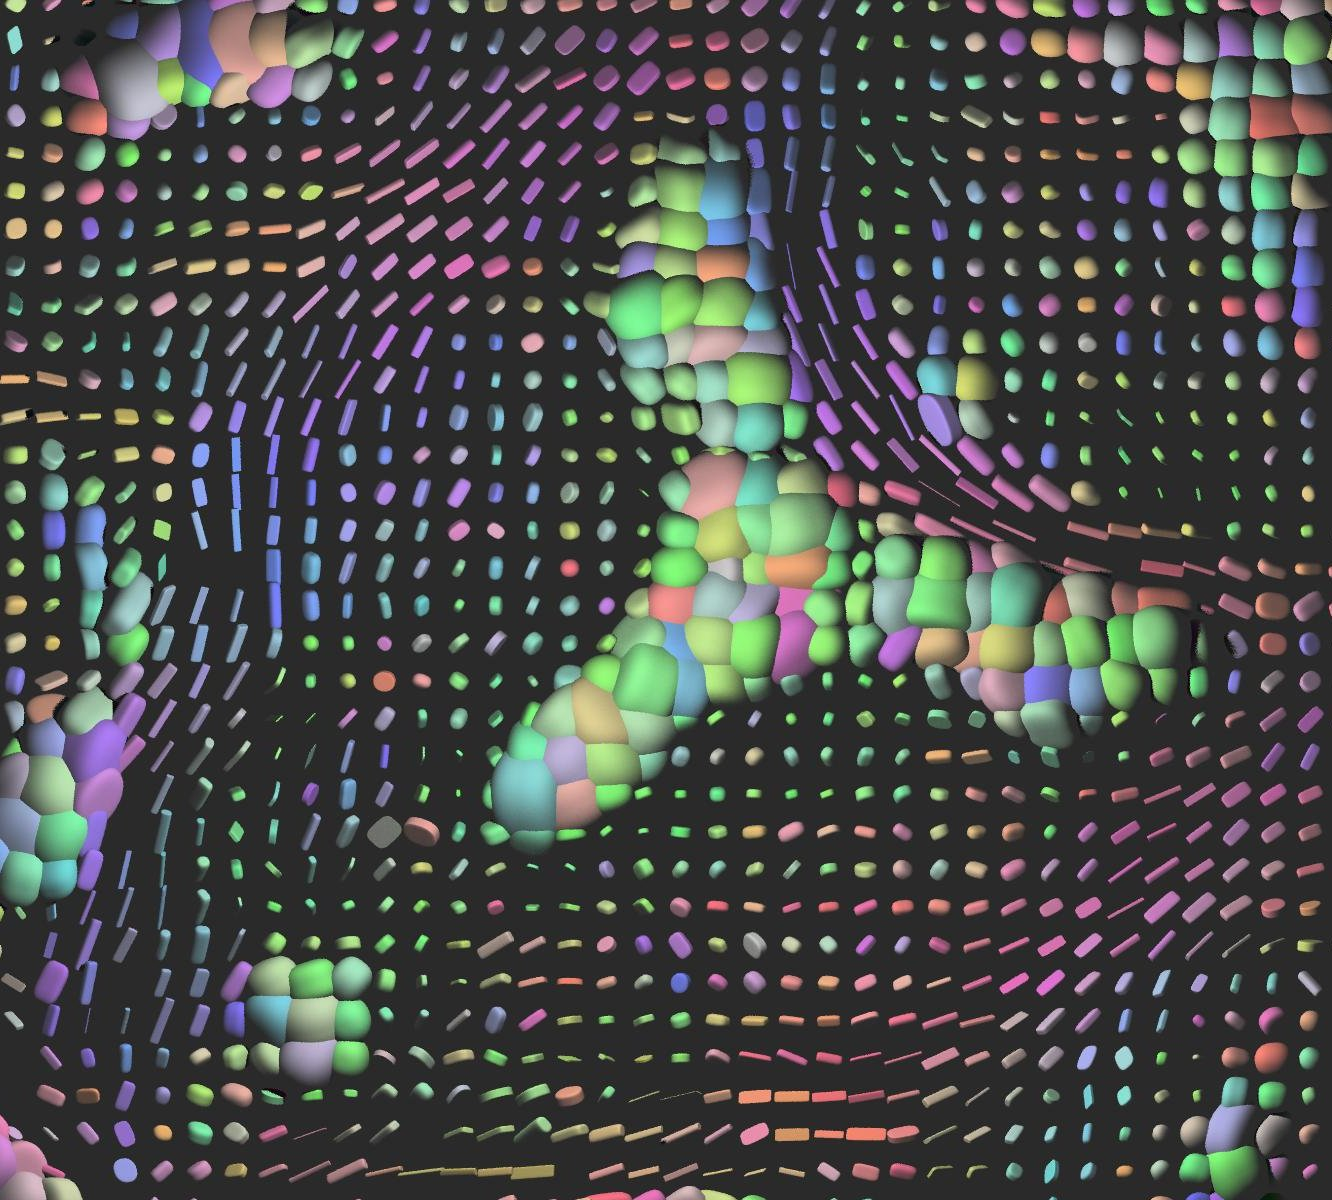
\includegraphics[width=.95\textwidth]{rotation45-zoomed-bs4-cropped.jpg}
\caption[Tensor Transformation]{Real DT image transformed with a $45^{\circ}$ rotation - Linear
interpolation.\\}
\label{fig:figure2}
\end{minipage}
\begin{minipage}[b]{0.5\linewidth}
\centering
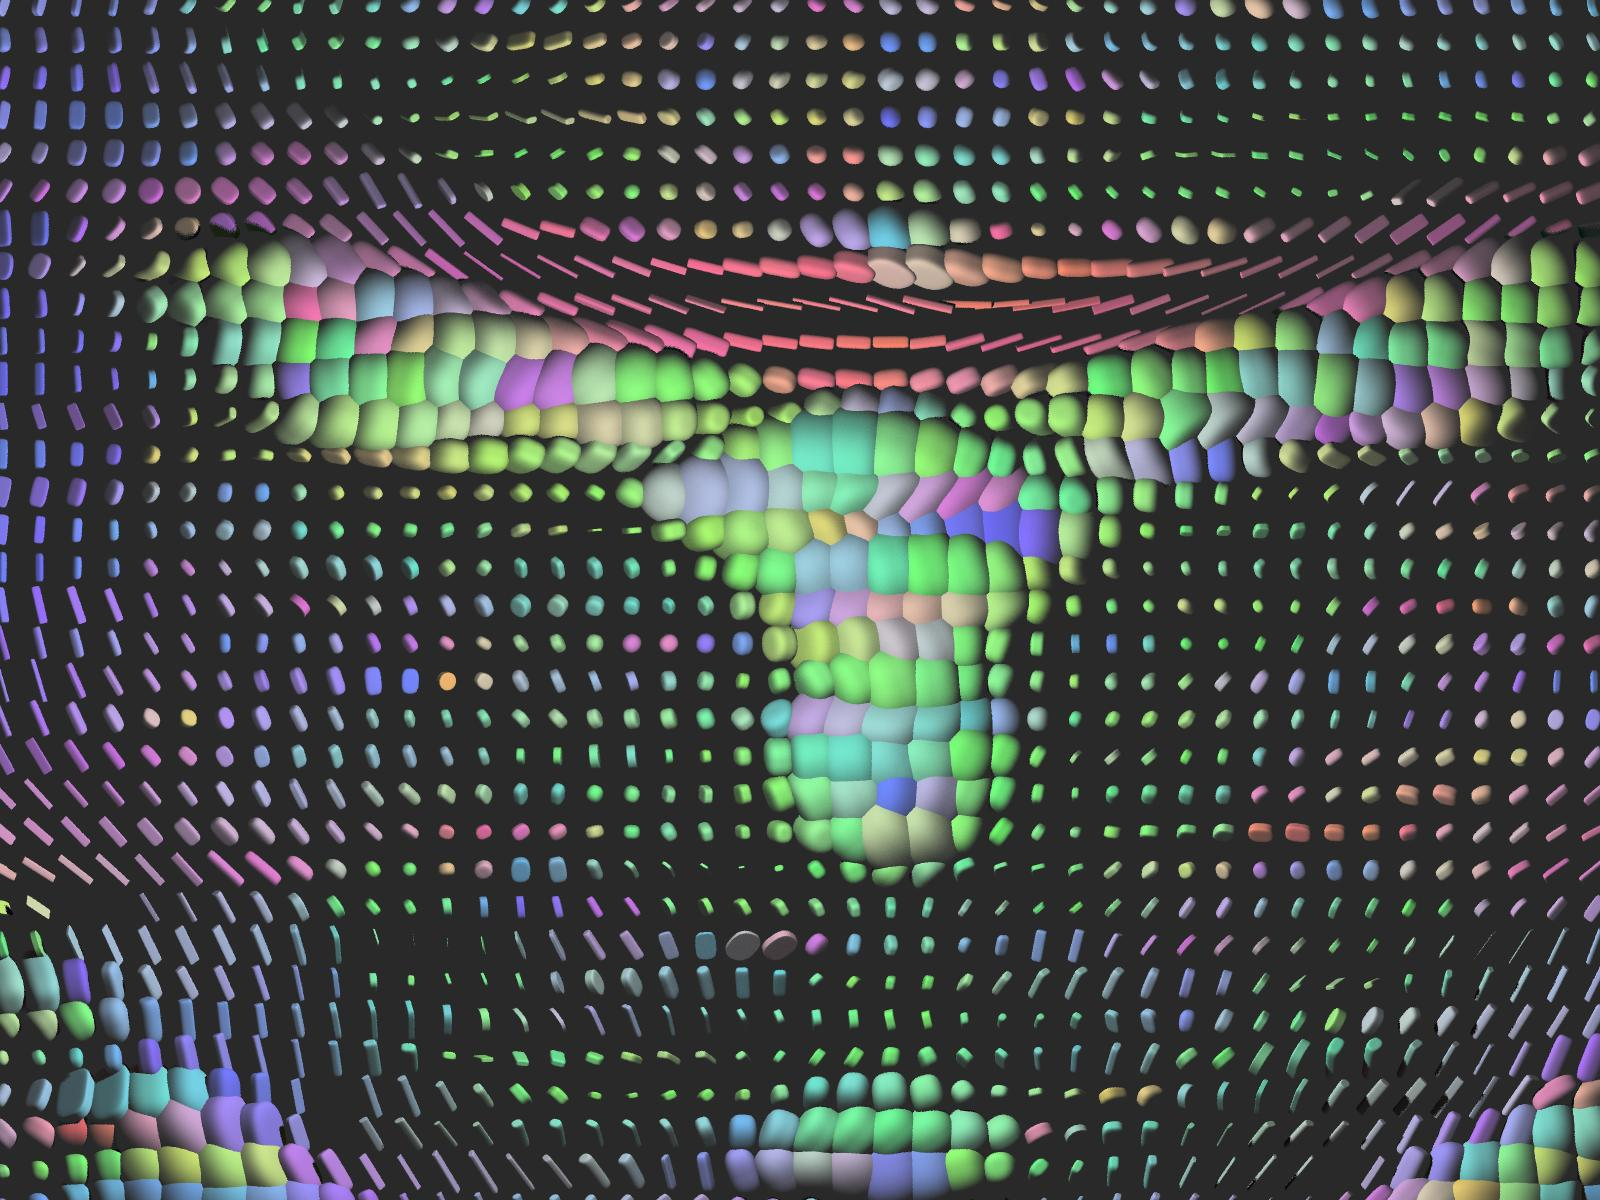
\includegraphics[width=.95\textwidth]{scale-zoomed.jpg}
\caption[Tensor Transformation]{Real DT image upscaled with a factor 2 - Linear
interpolation}
\label{fig:figure3}
\end{minipage}
\end{figure}
\clearpage
%Old real image insertion, one after the other
%\begin{figure}[!h]
%\center
%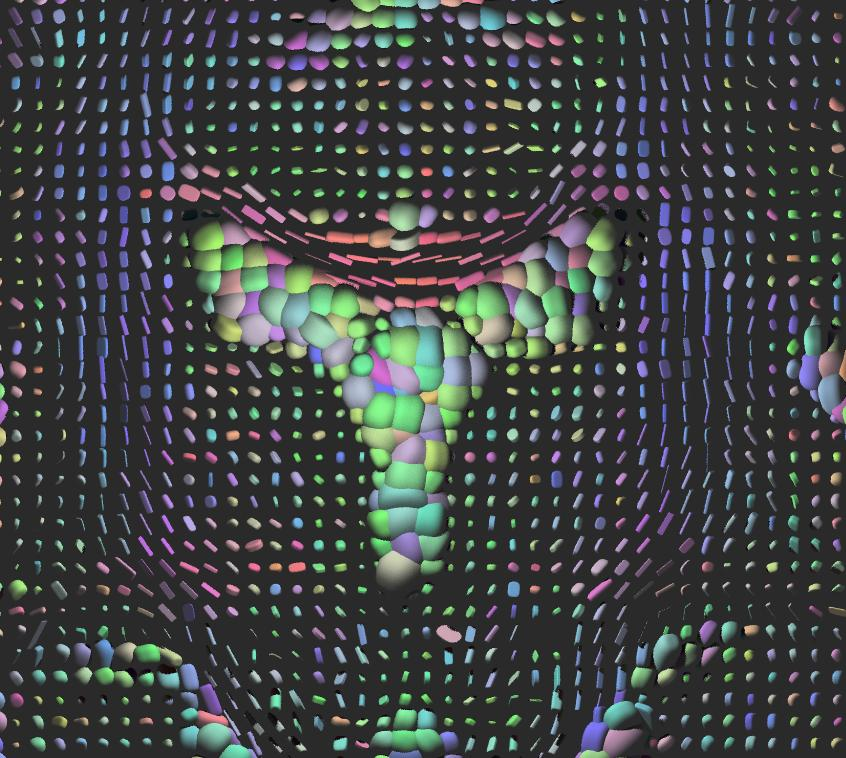
\includegraphics[width=0.55\textwidth]{OriginalSlice.jpg}
%\itkcaption[Tensor Transformation]{Slice extracted from a real DT image - No transformation.}
%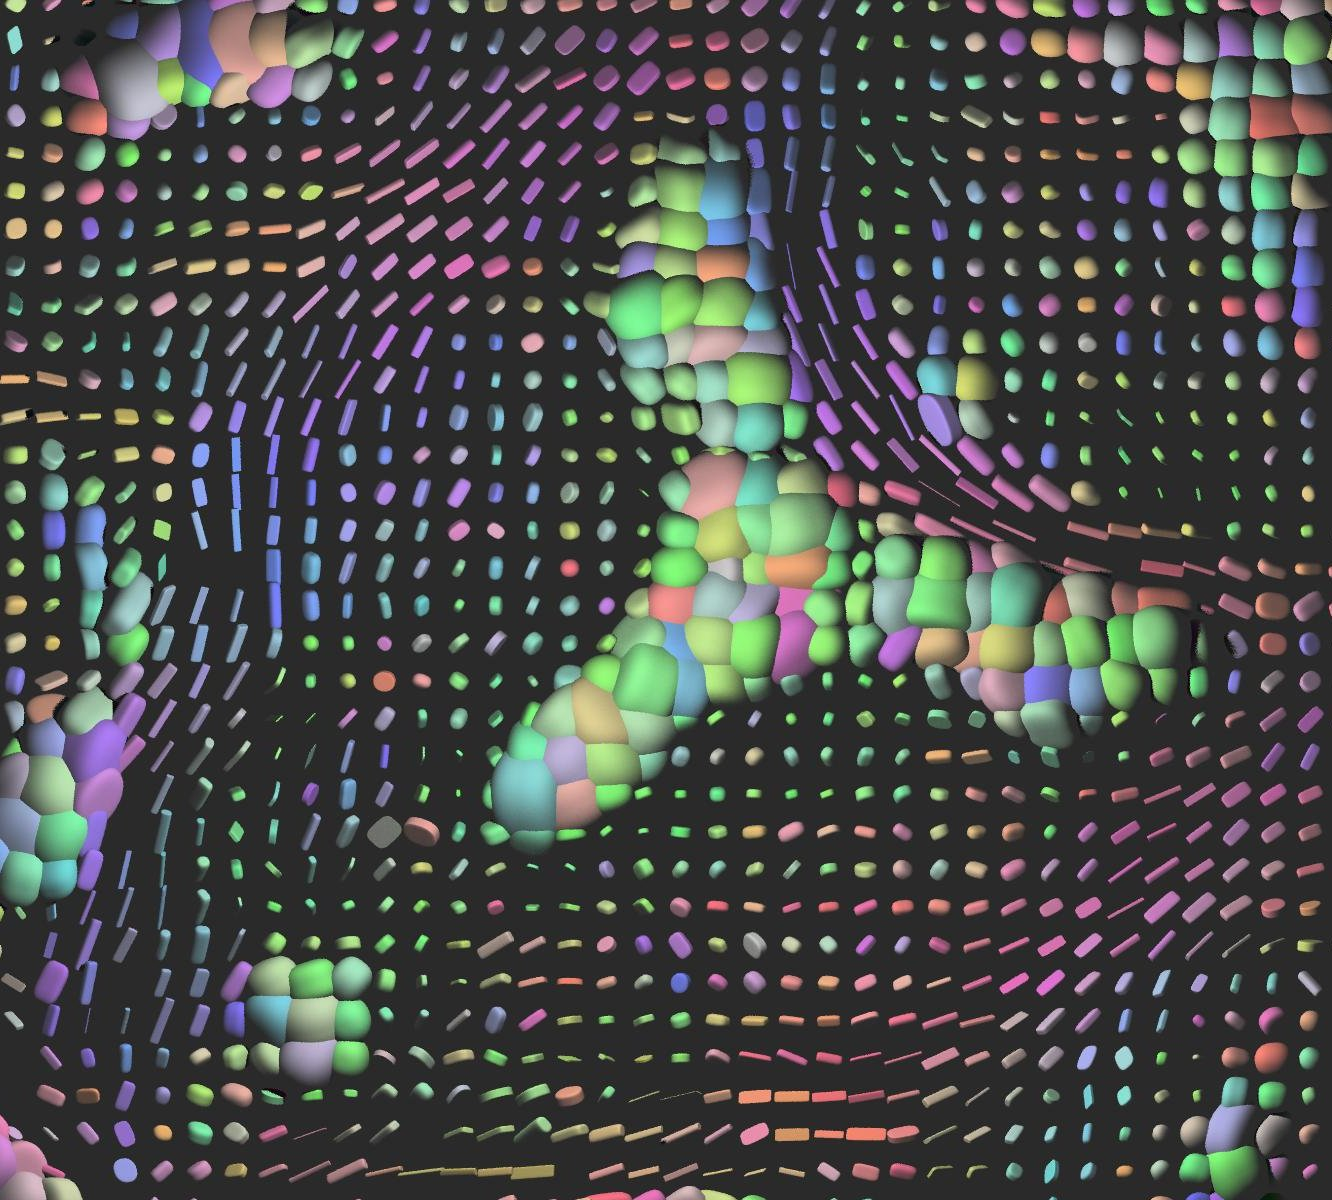
\includegraphics[width=0.55\textwidth]{rotation45-zoomed-bs4-cropped.jpg}
%\itkcaption[Tensor Transformation]{Real DT image transformed with a $45^{\circ}$ rotation.}
%\end{figure}

%%%%%%%%%%%%%%%%%%%%%%%%%%%%%%%%%%%%%%%%%
%
%  Insert the bibliography using BibTeX
%
%%%%%%%%%%%%%%%%%%%%%%%%%%%%%%%%%%%%%%%%%

\bibliographystyle{plain}
\bibliography{InsightJournal}


\end{document}

